\documentclass[ngerman]{fbi-aufgabenblatt}

\usepackage[shortlabels]{enumitem}
\usepackage{listings}
% Folgende Angaben bitte anpassen

\definecolor{dkgreen}{rgb}{0,0.6,0}
\definecolor{gray}{rgb}{0.5,0.5,0.5}
\definecolor{mauve}{rgb}{0.58,0,0.82}


\lstset{frame=tb,
  language=Java,
  aboveskip=3mm,
  belowskip=3mm,
  showstringspaces=false,
  columns=flexible,
  basicstyle={\small\ttfamily},
  numbers=left,
  numberstyle=\tiny\color{gray},
  keywordstyle=\color{blue},
  commentstyle=\color{dkgreen},
  stringstyle=\color{mauve},
  breaklines=true,
  breakatwhitespace=true,
  tabsize=3,
}

\renewcommand{\Vorlesung}{GSS}
\renewcommand{\Semester}{SoSe 2016}

\renewcommand{\Aufgabenblatt}{3}
\renewcommand{\Teilnehmer}{Chamier, Eickhoff, G�de, H�lzen, Jarsembinski}

\begin{document}
\section{Speicherverwaltung}
	\begin{enumerate}[(a)]
		\item Eine Seite setzt sich, wie in der Tabelle zu c, aus 4-Bit 
		Seitennummer, 3-Bit Seitenrahmennummer und 1-Bit f�r G�ltigkeit zusammen.
		Eine Seite ist also 8-Bit gro�.\\
		Die Adressen aus Teilaufgabe c) verwenden einen Offset von 12 Bit.
		Eine Kachel ist mit einem Offset von 12 Bit und einer Wortl�nge von 1 Byte 
		(8 Bit) $2^{12} \div 8 = 512 Bit = 64 Byte$ gro�. Eine Seite ist genau so gro�.\\		
		\item[(c)]
			\begin{enumerate}[i)]
			\item 001 1111 1110 1000 = 0x1FE8
			\item >Page Fault<
			\item 000 0100 0111 0000 = 0x0470
			\item 101 0001 0000 0001 = 0x5101				
			\end{enumerate}
		\item[(d)]
			Pro kleine Seitengr��e:
				\begin{enumerate}
					\item Mehr Kapazit�t f�r multiple Prozesse
					\item Effizientere Speichernutzung
				\end{enumerate}
			Pro gro�e Seitengr��e:
				\begin{enumerate}
					\item Weniger Aufwand bei Adressberechnung
				\end{enumerate}
		\item[(e)]
			Je kleiner die Seitentabellengr��e ist, desto weniger Seiten k�nnen referenziert werden 
			und desto gr��er sind die Seiten und Kacheln. Damit ist dann also der interne Speicher 
			weniger fragmentiert.\\
			Eine gute Seitengr��e f�r die durchschnittliche Prozessgr��e $p=4 MiB$ ist, durch 
			Ann�herung ermittelt, $1,6 MiB$. Mit dieser Seitengr��e belegt der durchschnittliche 
			Prozess 3 Seiten, wobei die letzte Seite halb leer bleibt. Kleinere Prozesse haben noch 
			einen gewissen Spielraum nach unten und gr��ere Prozesse m�ssen einfach mehr Seiten 
			verwenden.
	\end{enumerate}
\section{Seitenersetzungsalgorithmen}
 	\begin{enumerate}[a)]
 	\item \hspace{1pt}\\ 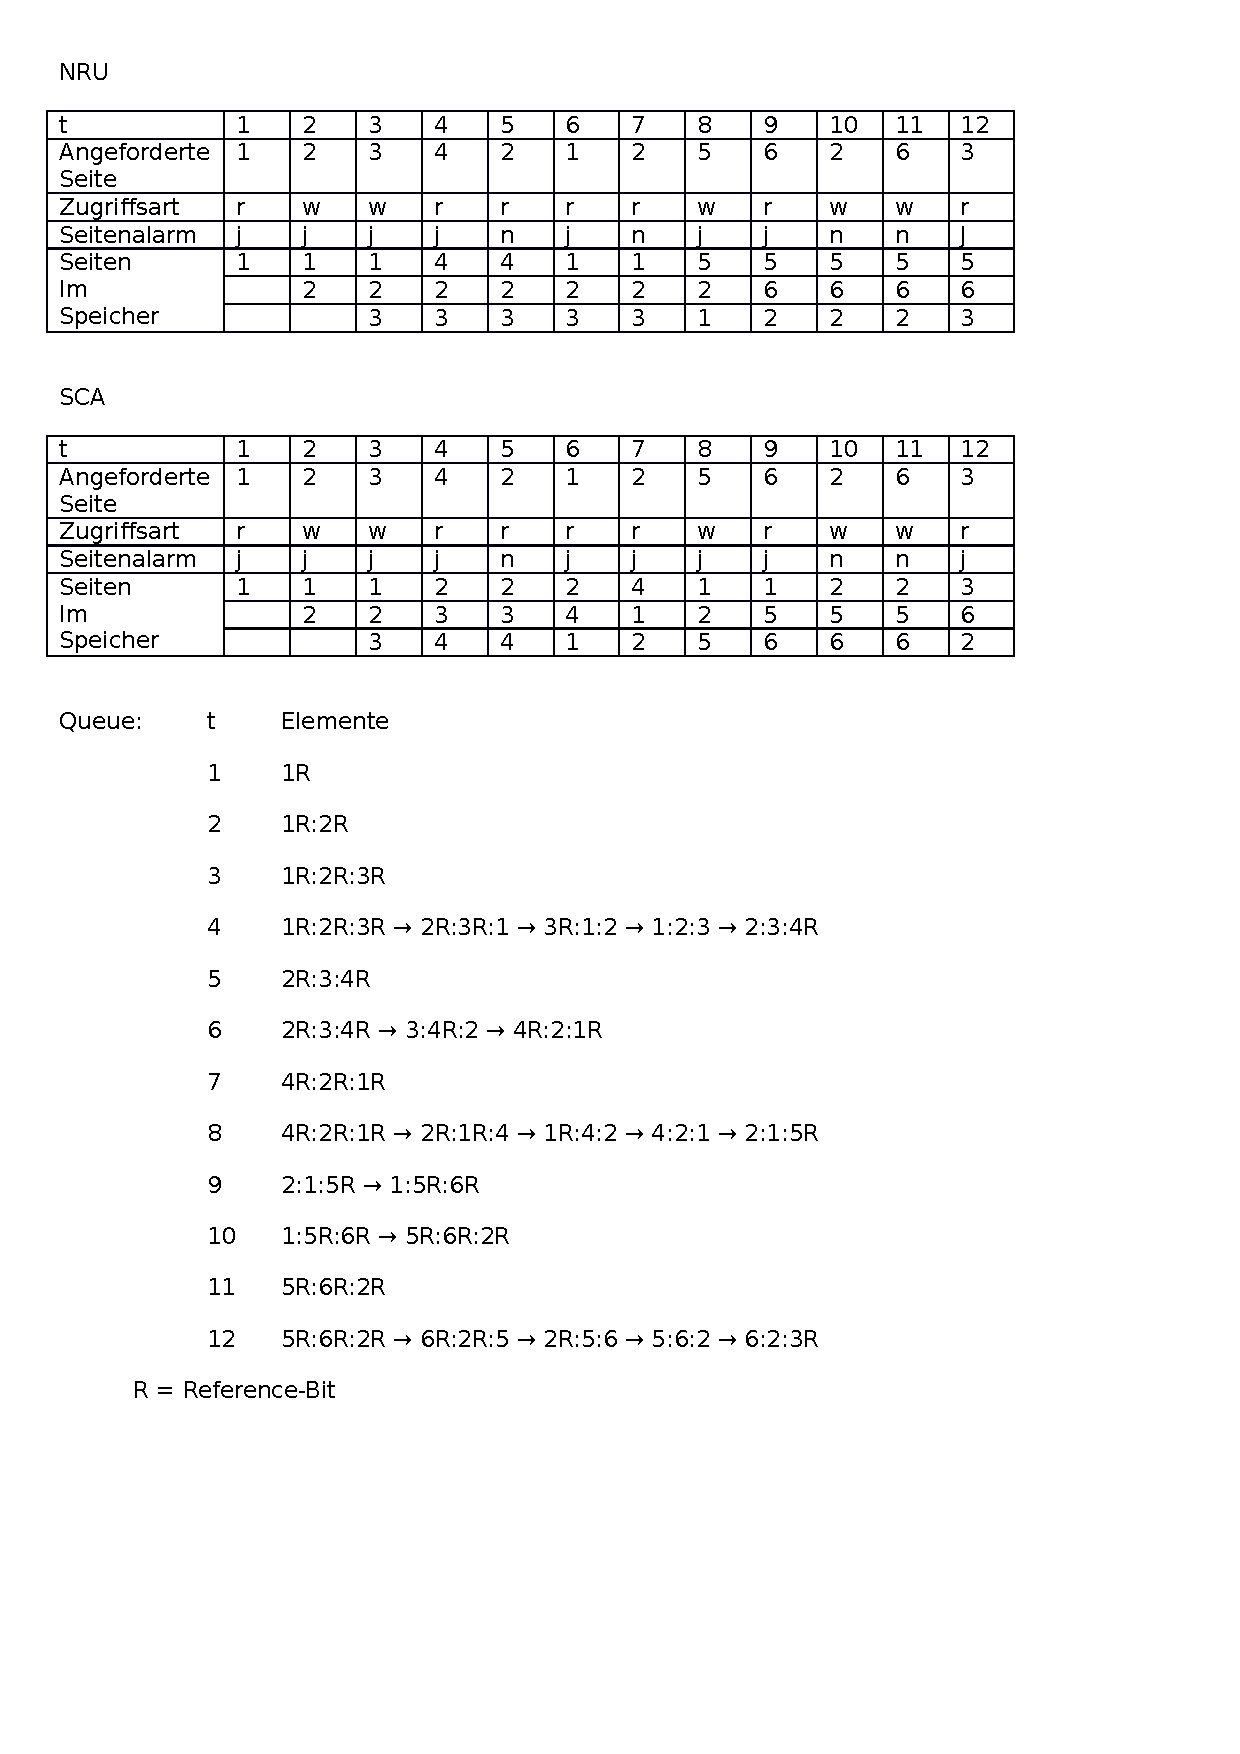
\includegraphics[scale=0.683]{Seitenverdraengung.pdf}
 	\end{enumerate}
\section{Synchronisation}
	\begin{enumerate}[a)] 
	\item 
		\lstinputlisting[language=python,caption=Semaphore.py]{Semaphore.py}
	\item 
		In obiger Implementation werden Prozesse, die schreibend auf die Daten zugreifen wollen,
		benachteiligt, da ''Reader'' unbegrenzt auf die Daten zugreifen k�nnen. Es w�re also m�glich,
		dass der schreibende Prozess niemals Zugriff bekommt, da immer neue ''Reader'' auf die Daten
		zugreifen. Um dies zu verhindern l�sst sich z.B. eine Queue einbauen, die Prozesse nur nach 
		und nach Zugriff auf die Daten erlaubt.
	\end{enumerate}
\end{document}
